% ==========================================================
% Archivo: chapters/ansible.tex
% Capítulo: Automatización del clúster con Ansible
% ==========================================================

\chapter{Automatización del clúster con Ansible}
\label{chap:ansible}

Este capítulo presenta Ansible como herramienta de automatización para administración de infraestructura. Primero se explica qué es, cómo funciona y cómo se organiza un proyecto típico. Después se muestran ejemplos independientes (no ligados todavía a la implementación del clúster). En la siguiente sección del capítulo se documenta la implementación realizada en la práctica para este proyecto.

% \begin{figure}[h]
%   \centering
%   \includegraphics[width=0.92\textwidth]{images/cap_ansible/a00_portada_capitulo.png}
%   \caption{Imagen introductoria del capítulo (opcional).}
%   \label{fig:ansible_intro}
% \end{figure}

\section{¿Qué es Ansible y por qué se usa en un clúster?}
\label{sec:ansible_que_es}

Ansible es una herramienta de automatización para administrar múltiples equipos de forma centralizada. En lugar de conectarse manualmente a cada nodo para repetir acciones (instalar paquetes, modificar archivos de configuración, habilitar servicios, montar directorios), Ansible permite describir esas acciones y ejecutarlas de manera consistente sobre un conjunto de equipos.

En un clúster, esta forma de trabajo es especialmente útil porque:
\begin{itemize}
  \item Reduce errores humanos al repetir procedimientos.
  \item Facilita mantener los nodos consistentes entre sí.
  \item Permite re-ejecutar configuraciones cuando un nodo se reinstala o se agrega un nuevo nodo.
\end{itemize}

Ansible es \textit{agentless}: no requiere instalar un ``agente'' permanente en los nodos administrados. En Linux, normalmente se conecta usando SSH desde un nodo de control hacia los nodos gestionados. \cite{rh_how_ansible_works,ansible_installation_guide}

\section{Cómo funciona Ansible}
\label{sec:ansible_como_funciona}

\subsection{Nodos y modelo de ejecución}
\label{subsec:ansible_nodos}

Ansible trabaja con dos roles principales:
\begin{itemize}
  \item \textbf{Nodo de control (control node):} equipo desde el cual se ejecutan los comandos y playbooks de Ansible.
  \item \textbf{Nodos gestionados (managed nodes):} equipos sobre los cuales se aplican las tareas.
\end{itemize}

En este proyecto, típicamente el \textit{master} cumple el rol de nodo de control para administrar los \textit{workers}. La comunicación ocurre por SSH y Ansible ejecuta módulos remotos (generalmente mediante Python en el nodo gestionado). \cite{ansible_installation_guide,rh_how_ansible_works}

\begin{figure}[H]
  \centering
  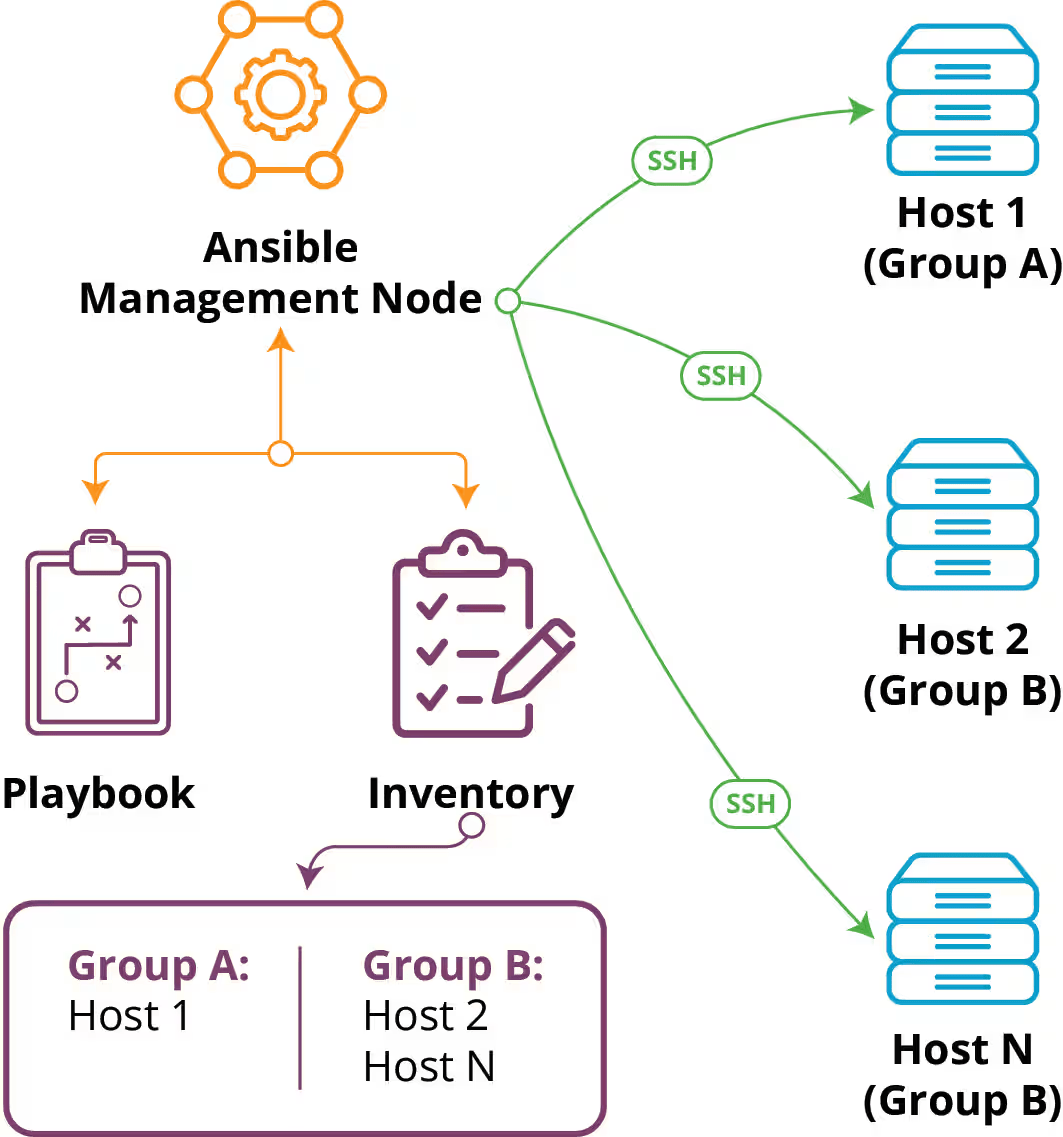
\includegraphics[width=0.5\textwidth]{images/ansible/Ansible diagrama.png}
  \caption{Esquema conceptual: nodo de control ejecutando tareas sobre nodos gestionados por SSH.}
  \label{fig:ansible_control_managed}
\end{figure}

\subsection{Inventario}
\label{subsec:ansible_inventario}

El \textbf{inventario} es la lista de equipos que Ansible administra y cómo se agrupan. Los formatos más comunes son INI y YAML. En el inventario se definen hosts, grupos (por ejemplo, \texttt{workers}) y variables de conexión. \cite{ansible_inventory_intro}

\subsection{Módulos, tareas y estado deseado}
\label{subsec:ansible_modulos}

Ansible ejecuta \textbf{módulos} (pequeñas unidades de trabajo) como ``instalar un paquete'', ``copiar un archivo'' o ``habilitar un servicio''. Muchos módulos están diseñados para ser \textbf{idempotentes}: si el estado deseado ya se cumple, no realizan cambios. Por eso, ejecutar el mismo playbook varias veces tiende a producir el mismo resultado final. \cite{ansible_modules_intro,ansible_playbooks_intro}

\subsection{Playbooks y roles}
\label{subsec:ansible_playbooks_roles}

Un \textbf{playbook} es un archivo YAML que describe qué tareas se ejecutan, sobre qué hosts, y con qué parámetros. Los playbooks se usan cuando la tarea se necesita repetir y versionar. \cite{ansible_playbooks_intro}

Un \textbf{rol (role)} organiza automatizaciones en una estructura reutilizable (tareas, variables, archivos y plantillas). Esto ayuda a mantener el proyecto ordenado cuando la automatización crece.

\section{Conceptos clave}
\label{sec:ansible_conceptos}

\begin{description}
  \item[Host pattern:] selección de objetivos, por ejemplo \texttt{all}, \texttt{master}, \texttt{workers}.
  \item[Variables:] parámetros para hacer playbooks reutilizables (por ejemplo, nombres de paquetes, rutas, puertos). \cite{ansible_variables}
  \item[Handlers:] acciones que se ejecutan solo si hubo un cambio (por ejemplo, reiniciar un servicio tras modificar su configuración). \cite{ansible_modules_intro}
  \item[Privilege escalation (become):] mecanismo para ejecutar tareas con privilegios elevados (similar a \texttt{sudo}). \cite{ansible_become}
\end{description}

\section{Requisitos mínimos para usar Ansible}
\label{sec:ansible_requisitos}

\subsection{En el nodo de control}
El nodo de control requiere Ansible instalado y un entorno Python compatible. \cite{ansible_installation_guide}

\subsection{En los nodos gestionados}
Los nodos gestionados no requieren Ansible instalado, pero normalmente requieren:
\begin{itemize}
  \item Acceso por SSH con una cuenta de usuario válida y un shell POSIX interactivo.
  \item Python para ejecutar el código que Ansible envía temporalmente al nodo (salvo excepciones como algunos módulos de red). \cite{ansible_installation_guide}
\end{itemize}

Por defecto, Ansible asume el uso de llaves SSH (recomendado). Si se usa contraseña, Ansible puede solicitarla con opciones específicas. \cite{ansible_connection_details}

\section{Ejemplos independientes de uso}
\label{sec:ansible_ejemplos}

Los ejemplos de esta sección sirven para entender el uso básico. En la implementación del proyecto se ajustan rutas, nombres de hosts, usuarios y llaves según el clúster.

\subsection{Ejemplo 1: inventario mínimo (INI)}
\label{subsec:ansible_ej1_inventario}

Un inventario INI mínimo define hosts y grupos:

\begin{verbatim}
# inventory.ini (ejemplo)
[master]
master ansible_host=10.195.34.17

[workers]
worker1 ansible_host=10.195.34.21
worker2 ansible_host=10.195.34.22

[all:vars]
ansible_user=sistemas
\end{verbatim}

Este formato permite apuntar a los hosts por nombre (\texttt{worker1}) y conservar la IP como variable (\texttt{ansible\_host}). \cite{ansible_inventory_intro}

% \begin{figure}[h]
%   \centering
%   \includegraphics[width=0.92\textwidth]{images/cap_ansible/a10_inventory_ini.png}
%   \caption{Ejemplo de inventario INI y su ubicación en el proyecto.}
%   \label{fig:ansible_inventory_ini}
% \end{figure}

\subsection{Ejemplo 2: comando ad hoc para probar conectividad (ping)}
\label{subsec:ansible_ej2_ping}

Los \textbf{ad hoc commands} son comandos de una sola tarea que se ejecutan sin escribir playbooks. Son útiles para pruebas rápidas. \cite{ansible_adhoc_intro}

\begin{verbatim}
ansible -i inventory.ini all -m ping
\end{verbatim}

Si la conectividad y credenciales son correctas, cada host responde con \texttt{pong}.

% \begin{figure}[h]
%   \centering
%   \includegraphics[width=0.92\textwidth]{images/cap_ansible/a11_ansible_ping.png}
%   \caption{Ejecución de \texttt{ansible -m ping} y salida esperada.}
%   \label{fig:ansible_ping}
% \end{figure}

\subsection{Ejemplo 3: ejecutar un comando simple en varios hosts}
\label{subsec:ansible_ej3_command}

\begin{verbatim}
ansible -i inventory.ini workers -m command -a "hostname"
\end{verbatim}

Este ejemplo consulta el hostname en todos los \textit{workers}. Para comandos que requieren shell (pipes, redirecciones), se usa el módulo \texttt{shell} con cuidado.

\subsection{Ejemplo 4: playbook mínimo (instalar un paquete)}
\label{subsec:ansible_ej4_playbook}

Un playbook describe tareas repetibles. Este ejemplo asegura que un paquete esté presente:

\begin{verbatim}
# install-tools.yml (ejemplo)
- name: Instalar herramientas básicas
  hosts: workers
  become: yes
  tasks:
    - name: Asegurar que htop esté instalado
      ansible.builtin.dnf:
        name: htop
        state: present
\end{verbatim}

La idempotencia implica que, si \texttt{htop} ya está instalado, la tarea no vuelve a instalarlo. \cite{ansible_playbooks_intro,ansible_modules_intro}

Para ejecutarlo:

\begin{verbatim}
ansible-playbook -i inventory.ini install-tools.yml
\end{verbatim}

% \begin{figure}[h]
%   \centering
%   \includegraphics[width=0.92\textwidth]{images/cap_ansible/a12_ansible_playbook_run.png}
%   \caption{Ejecución de un playbook con \texttt{ansible-playbook}.}
%   \label{fig:ansible_playbook_run}
% \end{figure}

\subsection{Ejemplo 5: copiar un archivo de configuración}
\label{subsec:ansible_ej5_copy}

\begin{verbatim}
# copy-example.yml (ejemplo)
- name: Copiar archivo a /etc
  hosts: master
  become: yes
  tasks:
    - name: Copiar un archivo de ejemplo
      ansible.builtin.copy:
        src: files/ejemplo.conf
        dest: /etc/ejemplo.conf
        owner: root
        group: root
        mode: "0644"
\end{verbatim}

Este tipo de automatización es útil para estandarizar configuraciones entre nodos.

\section{Implementación práctica en el clúster: instalación de Ansible y primera prueba}
\label{sec:ansible_practica_instalacion_ping}

Esta sección documenta la preparación del nodo de control y la primera prueba de conectividad con Ansible. En este proyecto, el nodo \textit{master} se usa como \textbf{nodo de control} para ejecutar automatizaciones sobre los \textit{workers}. Ansible se ejecuta desde el \textit{master} y se conecta a los demás nodos por SSH, lo que permite operar el clúster sin acceder manualmente nodo por nodo. \cite{ansible_installation_distros,ansible_connection_details}

\subsection{Instalación de Ansible en el nodo master (nodo de control)}
\label{subsec:ansible_install_master}

En sistemas tipo RHEL/Rocky, Ansible puede instalarse desde repositorios del sistema (por ejemplo, AppStream en RHEL 9) o desde repositorios comunitarios (como EPEL) dependiendo de la distribución y del paquete deseado. En entornos de servidores es común usar el gestor de paquetes del sistema para mantener actualizaciones y dependencias controladas. \cite{redhat_rhel9_ansible_core,ansible_installation_distros}

\subsubsection*{Procedimiento realizado}
\begin{enumerate}
  \item Se actualizó el sistema para aplicar parches antes de instalar herramientas:
\end{enumerate}

\begin{verbatim}
sudo dnf -y update
\end{verbatim}

% \begin{figure}[h]
%   \centering
%   \includegraphics[width=0.92\textwidth]{images/cap_ansible/p01_dnf_update_master.png}
%   \caption{Actualización del sistema en el master antes de instalar Ansible.}
%   \label{fig:p01_dnf_update_master}
% \end{figure}

\begin{enumerate}
  \setcounter{enumi}{1}
  \item Se instaló Ansible en el \textit{master} usando \texttt{dnf}:
\end{enumerate}

\begin{verbatim}
sudo dnf install ansible-core -y
\end{verbatim}

\begin{figure}[H]
  \centering
  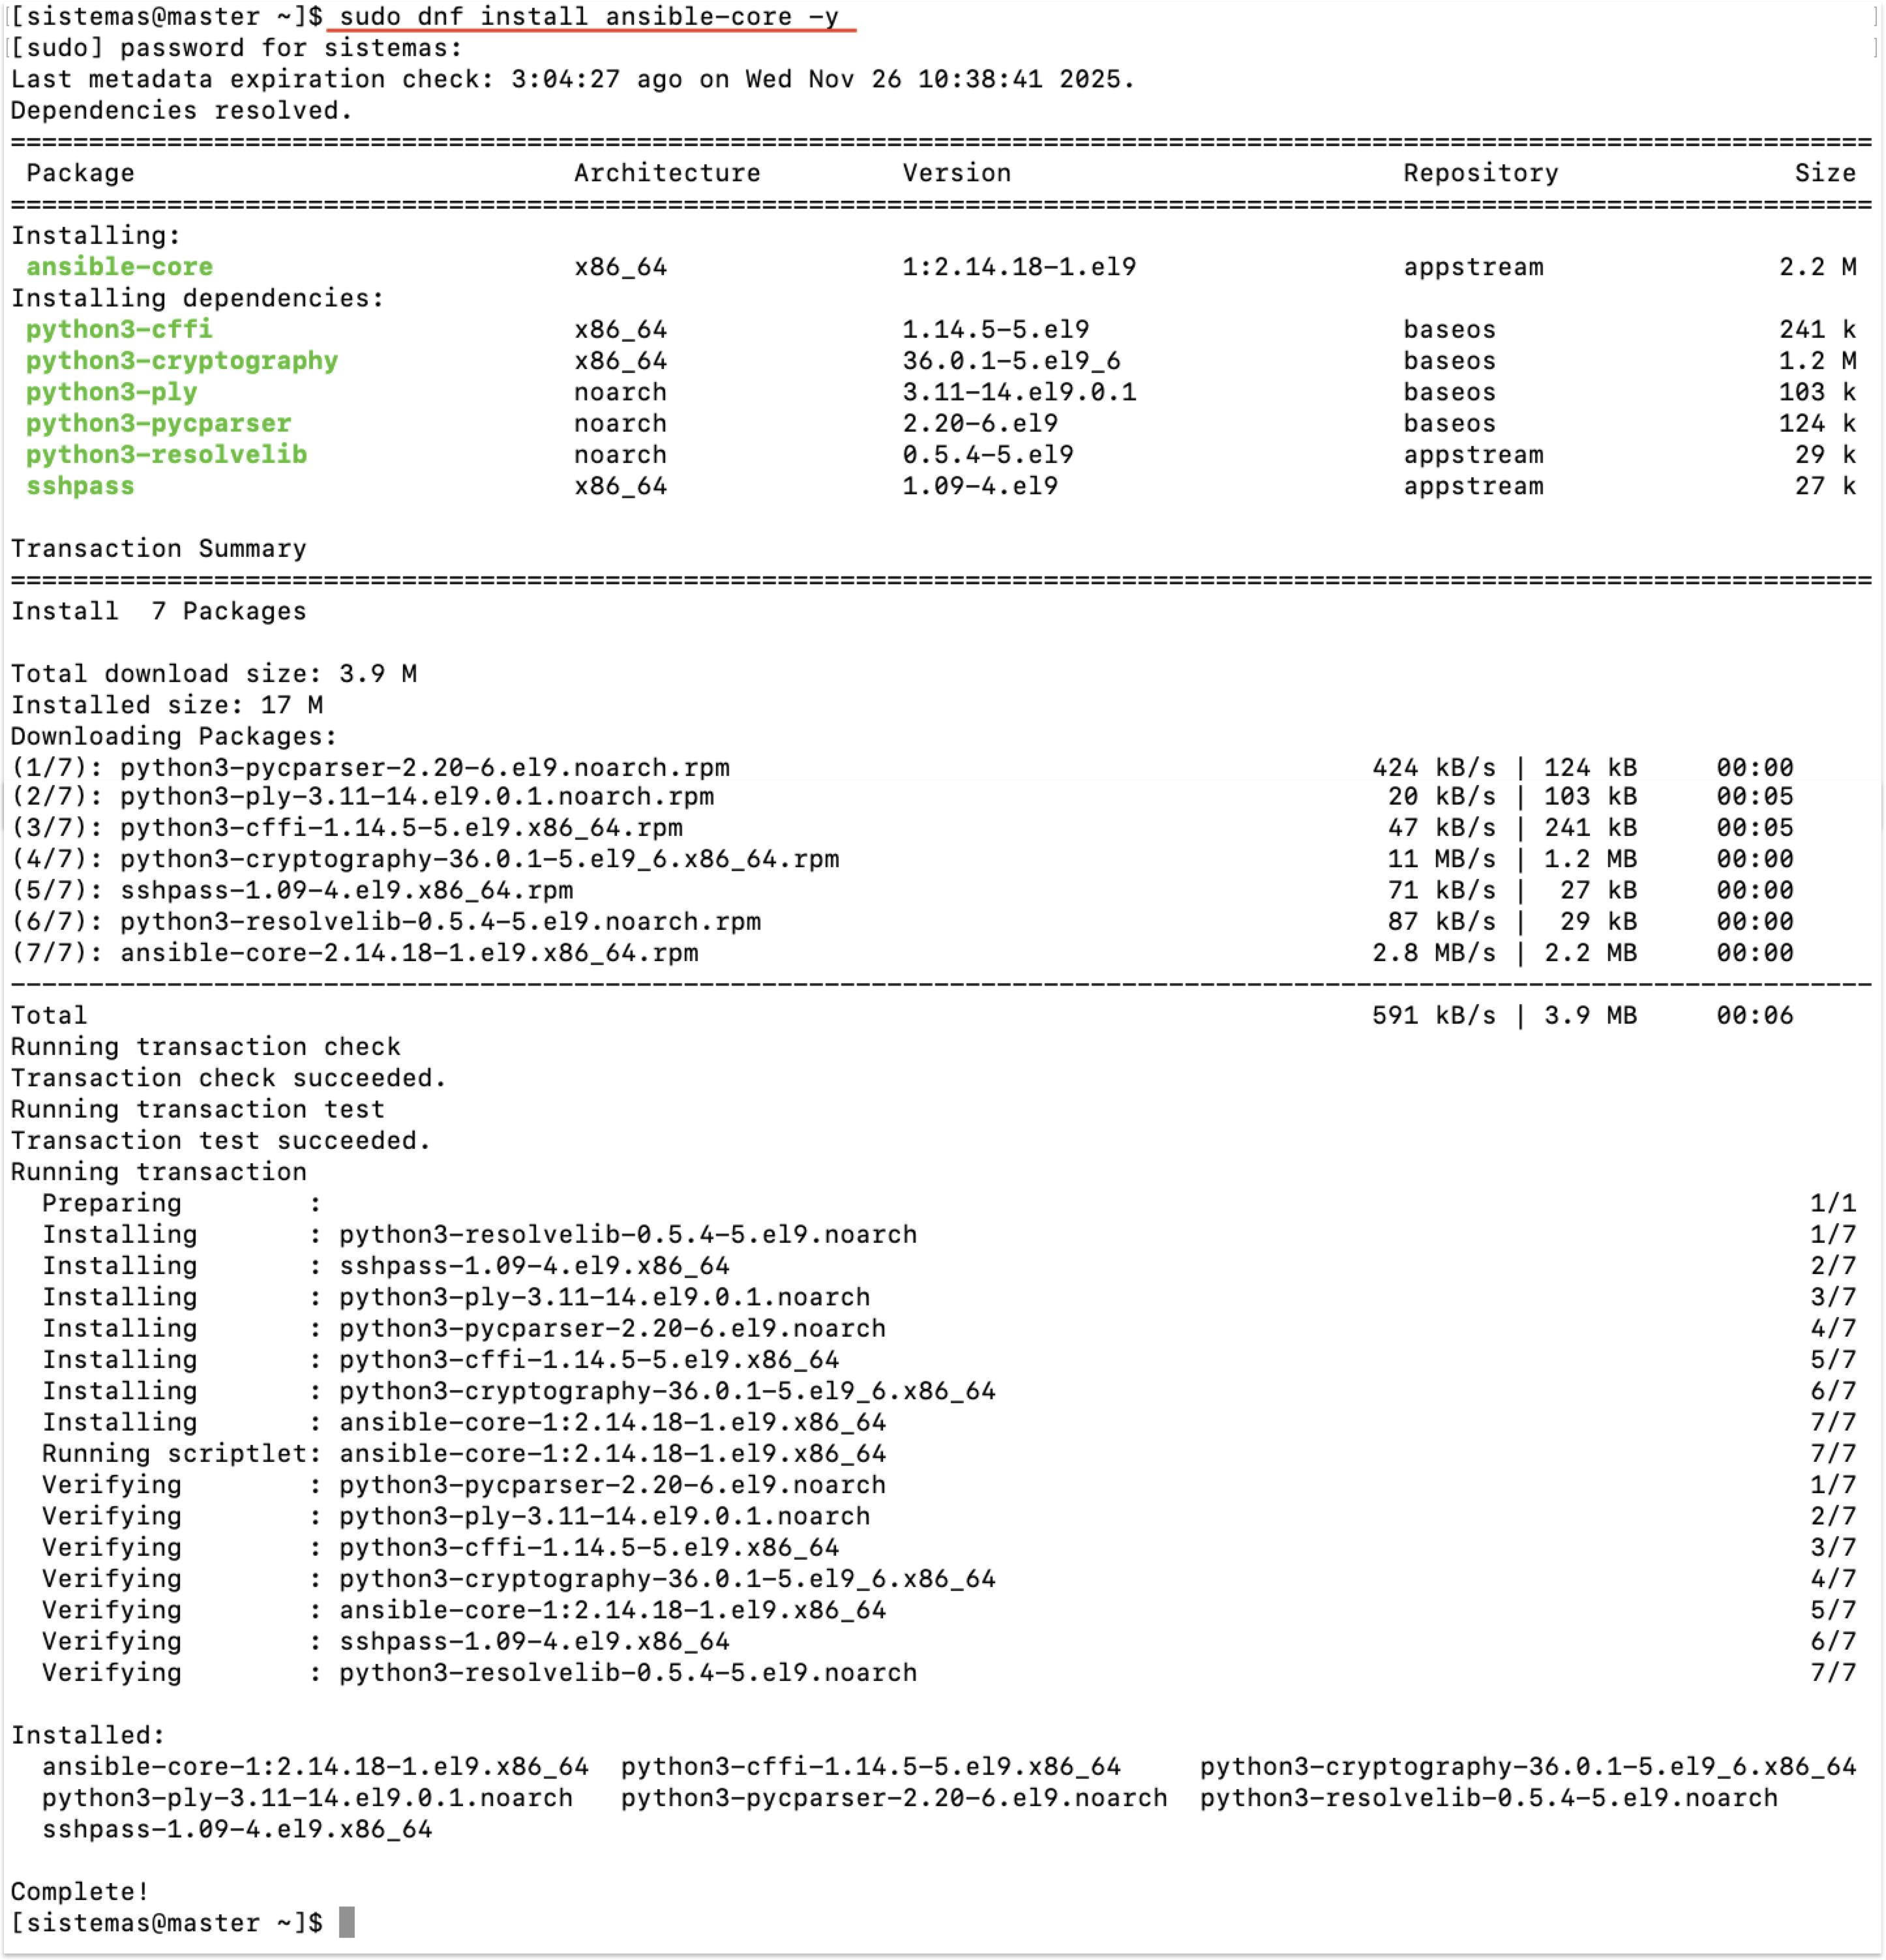
\includegraphics[width=0.6\textwidth]{images/ansible/ansible-core install.png}
  \caption{Instalación de Ansible (paquete \texttt{ansible-core}) en el master.}
  \label{fig:install_ansible_core}
\end{figure}

\begin{enumerate}
  \setcounter{enumi}{2}
  \item Se verificó la instalación y versión:
\end{enumerate}

\begin{verbatim}
ansible --version
\end{verbatim}

La salida mostró la versión de \texttt{ansible-core}, la versión de Python y la ruta del archivo de configuración de Ansible cuando aplica. Esto confirmó que Ansible quedó disponible desde la terminal del \textit{master}. \cite{ansible_installation_guide}

\begin{figure}[h]
  \centering
  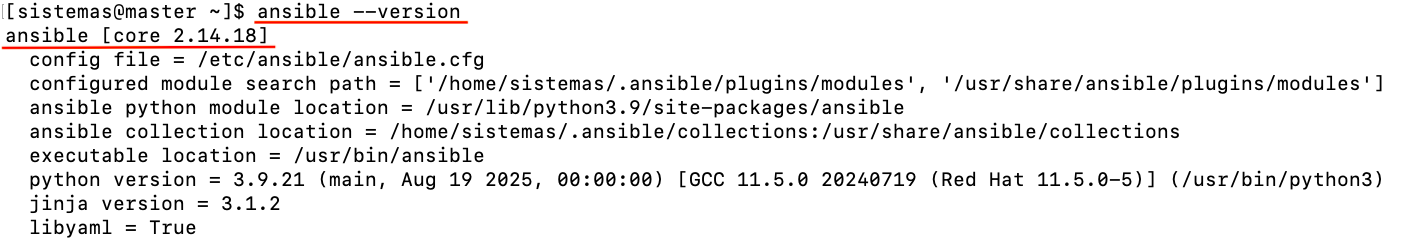
\includegraphics[width=0.92\textwidth]{images/ansible/ansible version.png}
  \caption{Verificación de instalación de Ansible con \texttt{ansible --version}.}
  \label{fig:p03_ansible_version}
\end{figure}

\subsection{Estructura mínima del proyecto de automatización}
\label{subsec:ansible_project_structure}

En este proyecto se organiza la automatización como un directorio de trabajo que contiene:
\begin{itemize}
  \item Un inventario (lista de hosts del clúster).
  \item Una configuración local del proyecto (\texttt{ansible.cfg}) para evitar depender de configuraciones globales.
  \item Playbooks y roles (cuando la automatización crece).
\end{itemize}

Mantener un \texttt{ansible.cfg} local ayuda a que el proyecto sea replicable: quien copie el repositorio obtiene la misma configuración por defecto. Ansible incluye herramientas para inspeccionar configuración y sus fuentes, como \texttt{ansible-config}. \cite{ansible_config_reference}

\subsubsection*{Procedimiento realizado}
\begin{enumerate}
  \item Se creó un directorio de trabajo para la automatización (ejemplo: \texttt{\textasciitilde/hpc-ansible}) y se ingresó a él:
\end{enumerate}

\begin{verbatim}
mkdir -p ~/hpc-ansible
cd ~/hpc-ansible
\end{verbatim}

\begin{figure}[H]
  \centering
  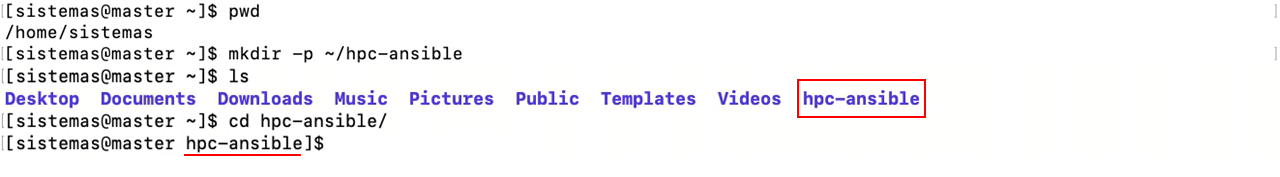
\includegraphics[width=0.92\textwidth]{images/ansible/dir ansible.png}
  \caption{Creación del directorio exclusivo para usar Ansible}
  \label{fig:p04_project_structure}
\end{figure}

\subsection{Creación del inventario del clúster (\texttt{inventario.ini})}
\label{subsec:ansible_inventory_ini_real}

El inventario define qué equipos administra Ansible y cómo conectarse a ellos. En este proyecto se organizó el inventario en dos grupos: \texttt{master} y \texttt{workers}. Además, se definió el usuario remoto común (\texttt{sistemas}) como variable global. \cite{ansible_inventory_intro,ansible_connection_details}

\subsubsection*{Procedimiento realizado}
\begin{enumerate}
  \item Se creó el archivo \texttt{inventario.ini} usando \texttt{nano}:
\end{enumerate}

\begin{verbatim}
nano inventario.ini
\end{verbatim}

En el editor se escribió el siguiente contenido y se guardó el archivo.

\begin{verbatim}
[hpc_master]
master ansible_host=10.195.34.17 ansible_user=sistemas

[workers]
worker1 ansible_host=10.195.20.52 ansible_user=sistemas
worker2 ansible_host=10.195.34.19 ansible_user=sistemas

[all:vars]
ansible_python_interpreter=/usr/bin/python3
ansible_ssh_private_key_file=~/.ssh/id_ed25519
\end{verbatim}

Para guardar en \texttt{nano} se usó \texttt{Ctrl+O}, luego \texttt{Enter}, y para salir \texttt{Ctrl+X}.

\begin{figure}[H]
  \centering
  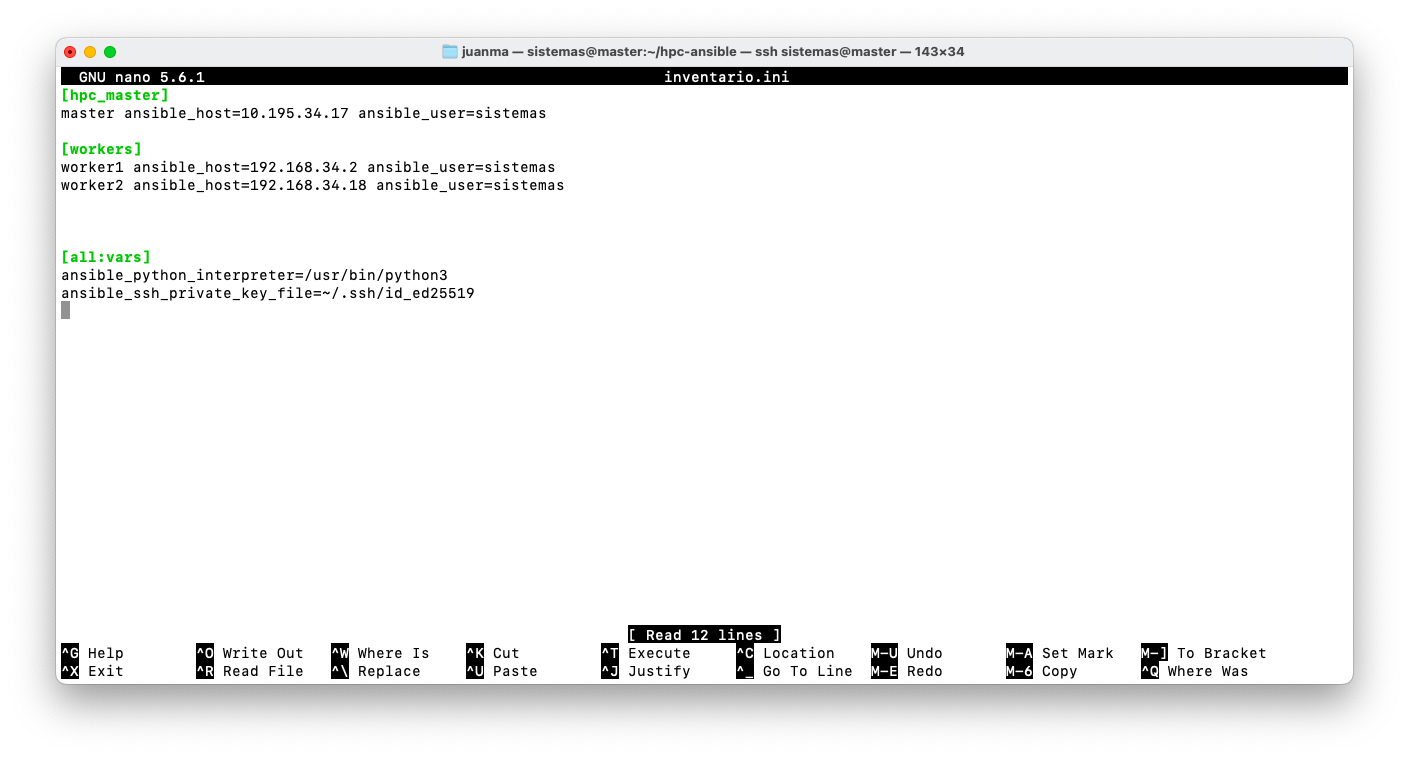
\includegraphics[width=0.92\textwidth]{images/ansible/inventario.png}
  \caption{Edición de \texttt{inventario.ini} con \texttt{nano}.}
  \label{fig:p05_inventory_ini_nano}
\end{figure}

En este punto, \texttt{worker1} y \texttt{worker2} pueden resolverse por nombre si existe DNS o si posteriormente se agregan entradas en \texttt{/etc/hosts}. Si aún no hay resolución de nombres, el inventario se completa asignando \texttt{ansible\_host=<IP>} a cada worker.

\subsection{Configuración local del proyecto (\texttt{ansible.cfg})}
\label{subsec:ansible_cfg_local_minimo}

Ansible permite definir parámetros por defecto en \texttt{ansible.cfg}. En esta fase se utiliza un archivo local para fijar el inventario por defecto y evitar escribir \texttt{-i inventory.ini} en cada comando. La referencia oficial documenta este comportamiento y las opciones disponibles. \cite{ansible_config_reference}

\subsubsection*{Procedimiento realizado}
\begin{enumerate}
  \item Se creó el archivo \texttt{ansible.cfg} usando \texttt{nano}:
\end{enumerate}

\begin{verbatim}
nano ansible.cfg
\end{verbatim}

En el editor se escribió el siguiente contenido y se guardó el archivo:

\begin{verbatim}
[defaults]
inventory = inventario.ini
timeout = 30

[ssh_connection]
pipelining = True
\end{verbatim}

\begin{figure}[H]
  \centering
  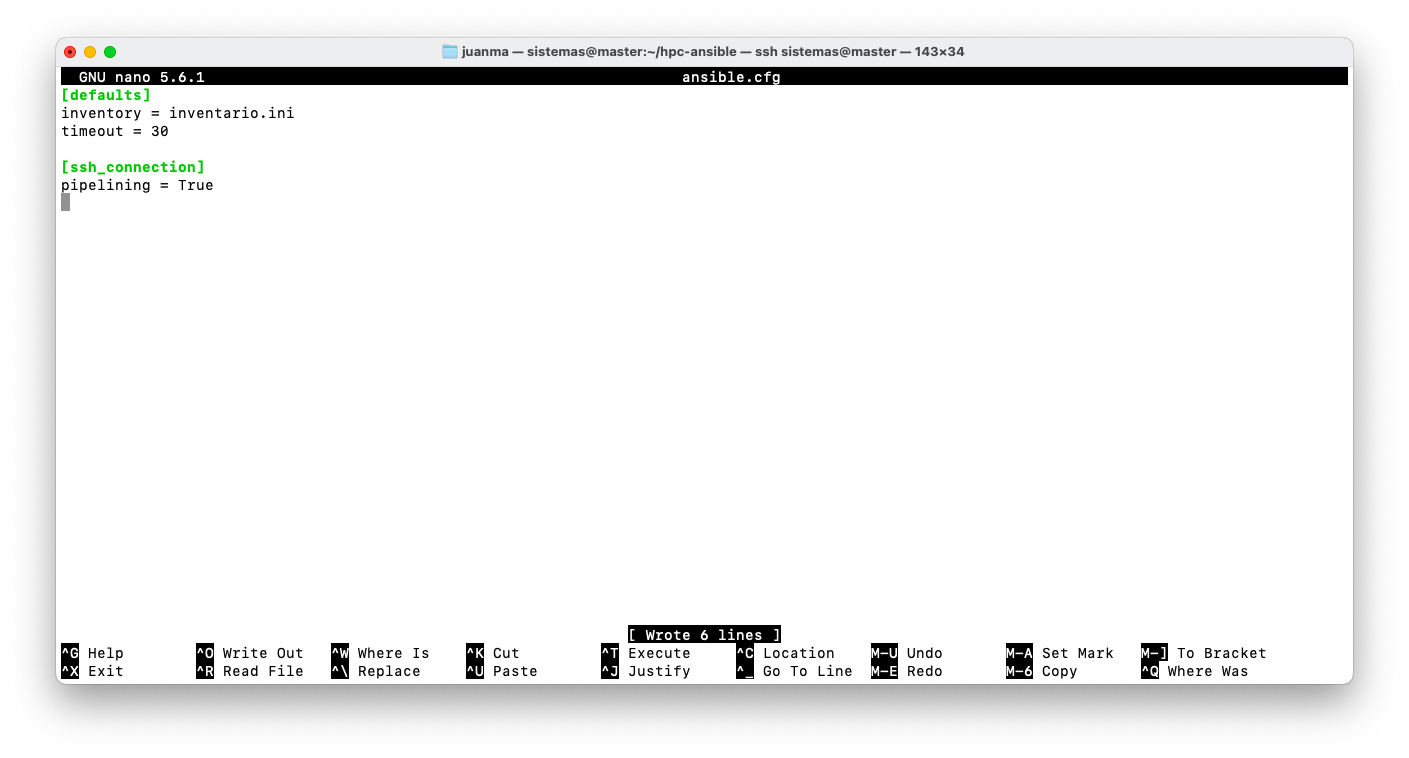
\includegraphics[width=0.92\textwidth]{images/ansible/ansible cfg.png}
  \caption{Edición de \texttt{ansible.cfg} con \texttt{nano}.}
  \label{fig:p06_ansible_cfg_nano}
\end{figure}

\begin{enumerate}
  \setcounter{enumi}{1}
  \item Se verificó que Ansible estuviera usando el archivo de configuración local:
\end{enumerate}

\begin{verbatim}
ansible --version
\end{verbatim}

En la salida se observó la línea \texttt{config file = .../hpc-ansible/ansible.cfg}, lo cual confirmó que la ejecución estaba tomando la configuración del proyecto.

\begin{figure}[H]
  \centering
  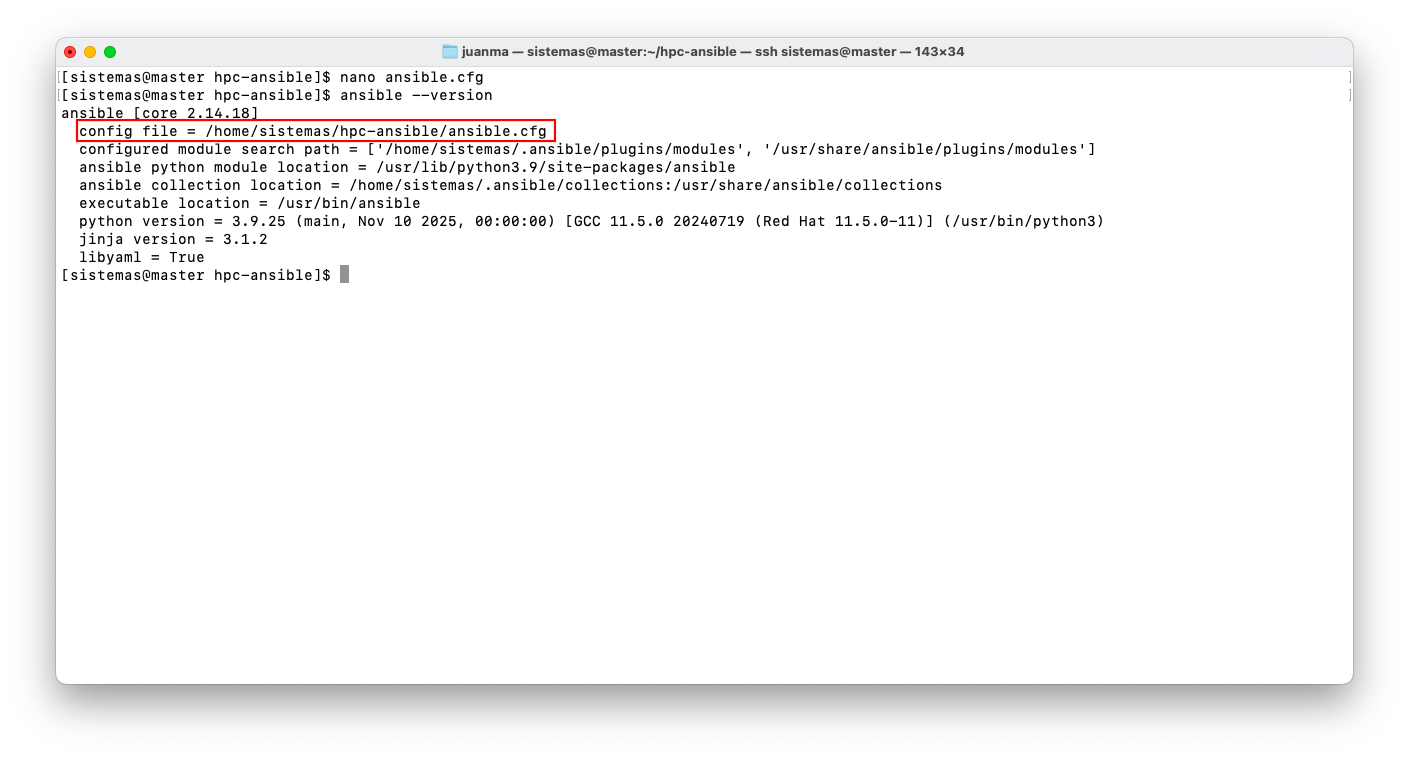
\includegraphics[width=0.92\textwidth]{images/ansible/ansible ver cfg.png}
  \caption{Verificación de \texttt{config file} en \texttt{ansible --version}.}
  \label{fig:p07_ansible_version_config_file}
\end{figure}

\subsection{Primera prueba de conectividad con Ansible}
\label{subsec:ansible_first_ping_minimo}

El módulo \texttt{ping} de Ansible se usa como prueba inicial porque confirma que el nodo de control puede conectarse al host remoto y ejecutar un módulo básico. Esta prueba depende de que exista conectividad SSH y credenciales correctas (preferiblemente llaves). \cite{ansible_adhoc_intro,ansible_connection_details}

\subsubsection*{Procedimiento realizado}
\begin{enumerate}
  \item Se probó conectividad contra todos los hosts del inventario:
\end{enumerate}

\begin{verbatim}
ansible all -m ping
\end{verbatim}

En la salida se observó \texttt{pong} en los hosts accesibles, lo cual confirmó que Ansible podía ejecutar módulos de forma remota.

\begin{figure}[H]
  \centering
  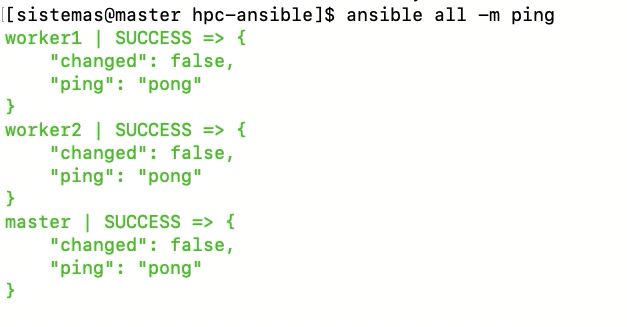
\includegraphics[width=0.75\textwidth]{images/ansible/all ping.png}
  \caption{Primera prueba con \texttt{ansible all -m ping} y respuesta \texttt{pong}.}
  \label{fig:p08_ansible_ping_all}
\end{figure}

\begin{enumerate}
  \setcounter{enumi}{1}
  \item Se verificó la identificación de los workers ejecutando \texttt{hostname}:
\end{enumerate}

\begin{verbatim}
ansible workers -m command -a "hostname"
\end{verbatim}

La salida mostró \texttt{worker1} y \texttt{worker2}, lo cual evidenció que las conexiones estaban llegando a los nodos correctos.

\begin{figure}[H]
  \centering
  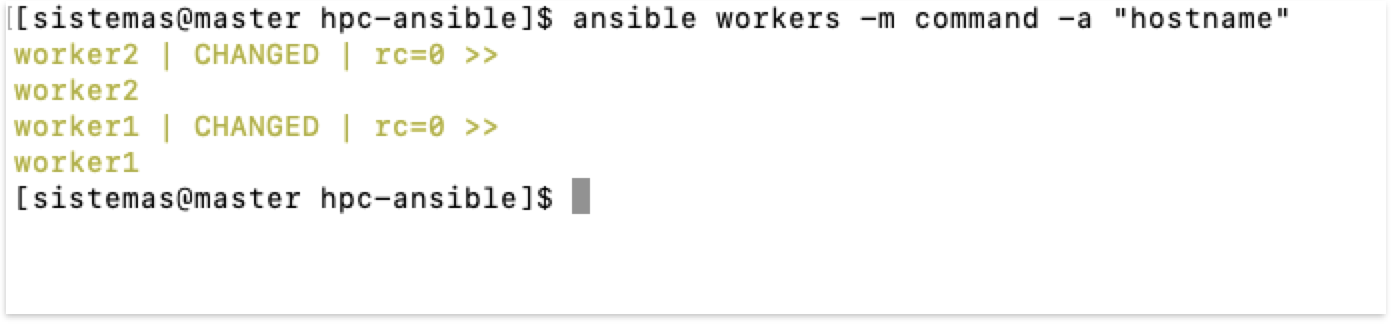
\includegraphics[width=0.92\textwidth]{images/ansible/ansible hostname workers.png}
  \caption{Ejecución del comando \texttt{hostname} en los workers con Ansible.}
  \label{fig:p09_ansible_hostname_workers}
\end{figure}

\section{YAML: el formato base de Ansible}
\label{sec:ansible_yaml}

Antes de describir playbooks, es útil entender \textbf{YAML}, el formato de texto con el que se escriben. YAML está pensado para ser legible por humanos, usando indentación para definir estructura. En Ansible, la mayoría de archivos clave (\texttt{site.yml}, playbooks, variables) están en YAML.

Conceptos mínimos de YAML:
\begin{itemize}
  \item \textbf{Indentación:} define jerarquías. Se recomienda usar dos espacios. No se mezclan tabs.
  \item \textbf{Listas:} comienzan con guion. Cada elemento es un ítem.
  \item \textbf{Mapas (pares clave-valor):} se escriben como \texttt{clave: valor}.
\end{itemize}

Ejemplo simple de YAML (lista de paquetes):
\begin{verbatim}
packages:
  - vim
  - git
  - htop
\end{verbatim}

Y ejemplo con mapas y listas combinadas:
\begin{verbatim}
server:
  name: nodo01
  services:
    - ssh
    - firewalld
\end{verbatim}

En Ansible, un playbook es una \textbf{lista} de \textit{plays}; por eso suele comenzar con un guion. La indentación y los guiones indican la estructura del documento. \cite{ansible_playbooks_intro}

\section{Playbooks, \textit{plays} y tareas (\textit{tasks})}
\label{sec:ansible_playbooks_plays_tasks}

Un \textbf{playbook} es el archivo YAML que describe una secuencia de acciones automatizables. Dentro de un playbook existen uno o varios \textbf{\textit{plays}}. Cada \textit{play} define \textit{qué hosts} se van a configurar, \textit{con qué permisos} y \textit{qué tareas} se ejecutan. Las \textbf{tareas (\textit{tasks})} son la unidad mínima de trabajo y normalmente invocan un módulo de Ansible para llevar un recurso a un estado deseado. \cite{ansible_playbooks_intro,ansible_modules_intro}

Componentes principales de un \textit{play}:
\begin{itemize}
  \item \textbf{name:} descripción en lenguaje natural. Aparece en la salida al ejecutar el playbook.
  \item \textbf{hosts:} grupo de equipos objetivo (por ejemplo, \texttt{all}, \texttt{hpc\_master}, \texttt{workers}).
  \item \textbf{become:} indica si se ejecuta con privilegios elevados (similar a \texttt{sudo}).
  \item \textbf{vars:} variables locales del \textit{play}. Permiten reutilizar el playbook.
  \item \textbf{tasks:} lista ordenada de tareas. Cada tarea invoca un módulo.
  \item \textbf{handlers:} acciones que se ejecutan solo si una tarea notificó cambios.
  \item \textbf{roles:} alternativa para declarar conjuntos de tareas empaquetadas.
\end{itemize}

Componentes principales de una \textit{task}:
\begin{itemize}
  \item \textbf{name:} descripción de la tarea.
  \item \textbf{módulo:} acción concreta (por ejemplo, \texttt{ansible.builtin.dnf}, \texttt{ansible.builtin.copy}).
  \item \textbf{parámetros:} argumentos del módulo, escritos en YAML.
  \item \textbf{notify:} opcional, dispara un \textit{handler} si hubo cambios.
\end{itemize}

Esta estructura permite separar responsabilidades: un \textit{play} puede dedicarse a configurar \textit{workers}, y otro a configurar el \textit{master}. A medida que el proyecto crece, se incorporan \textbf{roles} para encapsular conjuntos de tareas reutilizables.

\subsection{Ejemplo A: playbook con dos \textit{plays}}
\label{subsec:ansible_play_example_two_plays}

El siguiente ejemplo muestra un playbook con dos \textit{plays}: uno para tareas base en todos los nodos y otro específico para un grupo \texttt{web}.

\begin{verbatim}
# multi-play.yml (ejemplo)
- name: Preparar sistema base
  hosts: all
  become: yes
  tasks:
    - name: Ajustar zona horaria
      ansible.builtin.timezone:
        name: America/Bogota
    - name: Instalar paquetes base
      ansible.builtin.dnf:
        name:
          - vim
          - git
        state: present

- name: Configurar servidor web
  hosts: web
  become: yes
  tasks:
    - name: Instalar nginx
      ansible.builtin.dnf:
        name: nginx
        state: present
    - name: Habilitar y arrancar nginx
      ansible.builtin.systemd:
        name: nginx
        enabled: true
        state: started
\end{verbatim}

Aquí se observa que el primer \textit{play} es general (\texttt{all}) y el segundo se limita a un grupo específico (\texttt{web}). Cada \textit{play} puede tener sus propias tareas y variables.

\subsection{Ejemplo B: tareas con \textit{handlers}}
\label{subsec:ansible_play_example_handlers}

Un \textbf{\textit{handler}} es una tarea especial que \textbf{solo se ejecuta si alguna tarea anterior reporta cambios}. Se usa para acciones que no deben repetirse innecesariamente, como reiniciar o recargar un servicio.


Este ejemplo ilustra cómo una tarea puede disparar un \textit{handler} para reiniciar un servicio únicamente si hubo cambios en un archivo:

\begin{verbatim}
# config-app.yml (ejemplo)
- name: Desplegar configuración de una app
  hosts: app
  become: yes
  vars:
    app_port: 8080
  tasks:
    - name: Copiar plantilla de configuración
      ansible.builtin.template:
        src: templates/app.conf.j2
        dest: /etc/app/app.conf
      notify: Reiniciar servicio de app

  handlers:
    - name: Reiniciar servicio de app
      ansible.builtin.systemd:
        name: app
        state: restarted
\end{verbatim}

La relación entre tareas y \textit{handlers} es clave para mantener idempotencia y evitar reinicios innecesarios.

\section{Módulos de Ansible}
\label{sec:ansible_modulos}

Un \textbf{módulo} es la pieza que realiza el trabajo concreto dentro de una tarea. Cuando Ansible ejecuta una tarea, en realidad está llamando a un módulo que sabe cómo \textit{instalar un paquete}, \textit{copiar un archivo}, \textit{crear un usuario} o \textit{gestionar un servicio}. Los módulos están diseñados para ser \textbf{idempotentes}: si el estado deseado ya se cumple, no hacen cambios. \cite{ansible_modules_intro}

Componentes básicos de una tarea con módulo:
\begin{itemize}
  \item \textbf{name:} descripción de la acción.
  \item \textbf{módulo:} el nombre del módulo a ejecutar (por ejemplo, \texttt{ansible.builtin.dnf}).
  \item \textbf{parámetros:} opciones específicas del módulo (por ejemplo, nombre del paquete, estado).
\end{itemize}

Ejemplo de tarea usando un módulo:
\begin{verbatim}
- name: Asegurar que htop esté instalado
  ansible.builtin.dnf:
    name: htop
    state: present
\end{verbatim}

Otros módulos comunes:
\begin{itemize}
  \item \textbf{\texttt{ansible.builtin.copy}} para copiar archivos estáticos.
  \item \textbf{\texttt{ansible.builtin.template}} para generar archivos desde plantillas.
  \item \textbf{\texttt{ansible.builtin.systemd}} para habilitar o reiniciar servicios.
\end{itemize}

Comprender los módulos es clave porque cada uno tiene parámetros propios y resultados distintos. En capítulos posteriores se profundiza en los módulos más usados dentro del clúster.

\section{Playbook principal del proyecto (\texttt{site.yml}): estructura base}
\label{sec:ansible_site_base}

El archivo \texttt{site.yml} es el punto de entrada del proyecto de automatización. En esta etapa se presenta una \textbf{estructura base simplificada} que se irá completando a medida que avanzan los capítulos. Esta versión inicial permite entender la organización general sin entrar aún en todo el detalle.

\begin{verbatim}
# site.yml (estructura base inicial)
- name: Baseline para todos los nodos
  hosts: all
  become: true
  roles:
    - common
    # (se agregan más roles de base en capítulos posteriores)
\end{verbatim}

En los siguientes apartados se muestra cómo esta estructura se va enriqueciendo con roles adicionales hasta llegar a la versión actual del proyecto.


\section{Roles en Ansible}
\label{sec:ansible_roles}

Un \textbf{rol} es una forma de organizar la automatización en una estructura reutilizable y ordenada. En lugar de escribir todas las tareas dentro de un playbook, un rol agrupa tareas, variables, archivos y plantillas relacionadas con un objetivo específico (por ejemplo: \textit{firewall}, \textit{usuarios}, \textit{Slurm}).

Componentes típicos de un rol:
\begin{itemize}
  \item \textbf{\texttt{tasks/}}: lista de tareas principales del rol.
  \item \textbf{\texttt{defaults/}}: variables con valores por defecto (se pueden sobrescribir).
  \item \textbf{\texttt{vars/}}: variables internas del rol (prioridad más alta).
  \item \textbf{\texttt{handlers/}}: tareas especiales que se ejecutan solo si hubo cambios.
  \item \textbf{\texttt{templates/}}: archivos con plantillas Jinja2 para generar configuraciones.
  \item \textbf{\texttt{files/}}: archivos estáticos que se copian tal cual.
\end{itemize}

Cómo se usan los roles:
\begin{itemize}
  \item En un playbook se listan bajo \texttt{roles:} para aplicarlos a un grupo de hosts.
  \item Los roles se ejecutan en el orden en que aparecen.
  \item Las variables permiten adaptar el comportamiento del rol a cada entorno.
\end{itemize}

La ventaja principal es la \textbf{reutilización}: un rol bien definido puede usarse en distintos proyectos o aplicarse a varios grupos de hosts sin reescribir tareas.

\subsection{Ejemplo de rol: estructura y archivos clave}
\label{subsec:ansible_roles_ejemplo}

El siguiente ejemplo muestra un rol sencillo llamado \texttt{mi\_servicio}, con una estructura mínima típica. Se incluye un diagrama ASCII para visualizar las carpetas y dos archivos clave: uno de tareas y otro de \textit{handlers}.

\begin{verbatim}
roles/
└── mi_servicio/
    ├── tasks/
    │   └── main.yml
    ├── handlers/
    │   └── main.yml
    ├── defaults/
    │   └── main.yml
    ├── templates/
    │   └── mi_servicio.conf.j2
    └── files/
        └── banner.txt
\end{verbatim}

Ejemplo de \texttt{tasks/main.yml}:
\begin{verbatim}
# roles/mi_servicio/tasks/main.yml
- name: Instalar paquete del servicio
  ansible.builtin.dnf:
    name: mi-servicio
    state: present

- name: Desplegar configuración
  ansible.builtin.template:
    src: mi_servicio.conf.j2
    dest: /etc/mi_servicio/mi_servicio.conf
  notify: Reiniciar mi servicio
\end{verbatim}

Ejemplo de \texttt{handlers/main.yml}:
\begin{verbatim}
# roles/mi_servicio/handlers/main.yml
- name: Reiniciar mi servicio
  ansible.builtin.systemd:
    name: mi-servicio
    state: restarted
\end{verbatim}

Cómo funciona todo en conjunto:
\begin{itemize}
  \item El playbook invoca el rol \texttt{mi\_servicio} bajo la sección \texttt{roles:}.
  \item Ansible ejecuta las tareas de \texttt{tasks/main.yml} en orden.
  \item Si la tarea de plantilla modifica el archivo de configuración, se activa el \textit{handler}.
  \item El \textit{handler} reinicia el servicio solo cuando hubo cambios, evitando reinicios innecesarios.
\end{itemize}

\section{Variables, plantillas y archivos estáticos}
\label{sec:ansible_vars_templates_files}

Esta sección explica tres conceptos esenciales para hacer playbooks y roles flexibles: \textbf{variables}, \textbf{plantillas} y \textbf{archivos estáticos}. Cada uno cumple un propósito distinto, pero juntos permiten automatizar configuraciones reales sin repetir información.

\subsection{Variables}
\label{subsec:ansible_variables_intro}

Una \textbf{variable} es un valor que puede cambiar sin modificar el playbook. Sirve para parametrizar nombres de paquetes, rutas, puertos o usuarios. En Ansible, las variables se definen en diferentes lugares (por ejemplo, dentro del playbook, en \texttt{group\_vars/}, \texttt{host\_vars/} o en \texttt{defaults/} de un rol) y luego se usan con la sintaxis \texttt{\{\{ variable \}\}}. \cite{ansible_variables}

Ejemplo simple de variables en un playbook:
\begin{verbatim}
- name: Configurar un servicio con variables
  hosts: all
  become: yes
  vars:
    servicio: nginx
    puerto: 8080
  tasks:
    - name: Instalar servicio
      ansible.builtin.dnf:
        name: "{{ servicio }}"
        state: present
\end{verbatim}

En este ejemplo, cambiar \texttt{servicio} o \texttt{puerto} modifica el comportamiento del playbook sin reescribir tareas.

\subsection{Plantillas (Jinja2)}
\label{subsec:ansible_templates_intro}

Una \textbf{plantilla} es un archivo de texto que incluye variables y lógica básica para generar configuraciones dinámicas. Ansible utiliza el motor \textbf{Jinja2} para reemplazar variables y crear un archivo final en el host remoto. El módulo más común es \texttt{ansible.builtin.template}.

Las variables que aparecen en una plantilla provienen de las mismas fuentes que en un playbook: pueden estar definidas en \texttt{vars:} dentro del playbook, en archivos de grupo (\texttt{group\_vars/}), en archivos por host (\texttt{host\_vars/}) o en los \texttt{defaults/} de un rol. Al ejecutar el playbook, Ansible construye un conjunto de variables disponible para la plantilla y reemplaza cada \texttt{\{\{ variable \}\}} con su valor correspondiente. \cite{ansible_variables}

Ejemplo de plantilla (\texttt{templates/app.conf.j2}):
\begin{verbatim}
# app.conf.j2 (ejemplo)
port={{ puerto }}
log_path={{ log_dir }}/app.log
\end{verbatim}

Ejemplo de tarea que renderiza la plantilla:
\begin{verbatim}
- name: Generar configuración desde plantilla
  ansible.builtin.template:
    src: templates/app.conf.j2
    dest: /etc/mi_app/app.conf
\end{verbatim}

Si cambian las variables \texttt{puerto} o \texttt{log\_dir}, el archivo generado será diferente. Esto permite mantener una sola plantilla para múltiples nodos con configuraciones específicas.

\subsection{Archivos estáticos}
\label{subsec:ansible_static_files}

Un \textbf{archivo estático} es un archivo que se copia exactamente igual al host remoto, sin reemplazo de variables. Se usa para binarios, scripts, certificados, o archivos de texto que no requieren personalización. El módulo típico es \texttt{ansible.builtin.copy}, y los archivos suelen vivir en la carpeta \texttt{files/} del rol.

Ejemplo de tarea con archivo estático:
\begin{verbatim}
- name: Copiar banner estático
  ansible.builtin.copy:
    src: banner.txt
    dest: /etc/issue
    owner: root
    group: root
    mode: "0644"
\end{verbatim}

Es importante que la ruta de destino exista en los nodos de destino (por ejemplo, \texttt{/etc/} o \texttt{/opt/mi\_app/}). Si el directorio no existe, la tarea fallará, por lo que normalmente se crea antes con un módulo como \texttt{ansible.builtin.file}.

\section{Ejecución de playbooks y lectura de resultados}
\label{sec:ansible_ejecucion_playbooks}

Una vez escrito un playbook, se ejecuta con el comando \texttt{ansible-playbook}. El objetivo es que Ansible lea el archivo, se conecte a los hosts definidos en el inventario, ejecute las tareas en orden y reporte el resultado de cada una.

Comando general de ejecución:
\begin{verbatim}
ansible-playbook -i inventory.ini mi-playbook.yml
\end{verbatim}

Componentes del comando:
\begin{itemize}
  \item \textbf{\texttt{ansible-playbook}}: ejecuta playbooks.
  \item \textbf{\texttt{-i inventory.ini}}: indica el inventario a usar.
  \item \textbf{\texttt{mi-playbook.yml}}: el archivo con los \textit{plays} y tareas.
\end{itemize}

Si el proyecto ya tiene un \texttt{ansible.cfg} con el inventario por defecto, la opción \texttt{-i} puede omitirse. También es común usar \texttt{--limit} para restringir la ejecución a un host o grupo (por ejemplo, un solo worker durante pruebas).

\subsection{¿Qué muestra la salida de Ansible?}
\label{subsec:ansible_output}

Durante la ejecución, Ansible imprime una línea por cada tarea, junto con su estado. Los estados más comunes son:
\begin{itemize}
  \item \textbf{\texttt{ok}}: la tarea ya estaba en el estado deseado y no hubo cambios.
  \item \textbf{\texttt{changed}}: la tarea realizó cambios en el sistema.
  \item \textbf{\texttt{failed}}: la tarea falló (se detiene la ejecución salvo que se indique lo contrario).
  \item \textbf{\texttt{skipped}}: la tarea se omitió por una condición o por \texttt{--limit}.
\end{itemize}

Al final, Ansible muestra un resumen (\textit{play recap}) por cada host, indicando cuántas tareas fueron \texttt{ok}, \texttt{changed}, \texttt{failed}, \texttt{skipped}, \texttt{rescued} e \texttt{ignored}. Este resumen permite validar rápidamente si la ejecución fue correcta.

\subsection{Resultado esperado}
\label{subsec:ansible_expected_results}

En una ejecución exitosa, se espera:
\begin{itemize}
  \item Conectividad estable con todos los hosts del inventario.
  \item Cero fallos (\texttt{failed=0}) en el resumen final.
  \item Cambios solo cuando son necesarios (idempotencia).
\end{itemize}

Si se ejecuta el mismo playbook por segunda vez sin modificar nada, la mayoría de tareas deberían aparecer como \texttt{ok} y no \texttt{changed}, lo cual indica que el sistema ya está en el estado deseado.
